% vim: ai sw=2 spell spelllang=cs

\begin{frame}
  \frametitle{DWARF}

  \begin{itemize}
    \item Strukturované ladicí informace
    \begin{itemize}
      \item Zápis komplikovaných výrazů
      \begin{itemize}
	\item \code{void klist_init(struct klist *k, void (*get)(struct
	  klist_node *), void (*put)(struct klist_node *));}
      \end{itemize}

      \pause

      \item Vytvářené překladačem
    \end{itemize}

    \item Nezávislost na jazyku a formátu souborů

    \pause

    \item Dokumentace
    \begin{itemize}
      \item \href{http://www.dwarfstd.org/doc/Debugging\%20using\%20DWARF.pdf}{Introduction to the DWARF Debugging Format} (10 stran, obrázky)
      \item \href{http://www.dwarfstd.org/doc/DWARF4.pdf}{DWARF Debugging Information Format (Version 4)} ($>$ 300 stran)
    \end{itemize}

  \end{itemize}

\end{frame}

\begin{frame}
  \frametitle{DWARF formát}

  \begin{itemize}
    \item Ladicí informace v lese skoro-stromů
    \begin{itemize}
      \item Pro každý zdrojový soubor jeden skoro-strom
    \end{itemize}

    \pause

    \item Uzly stromů jsou \emph{Debugging Information Entry} (DIE)

    \pause

    \item Jeden DIE může odkazovat na kterýkoliv jiný
  \end{itemize}

  \onslide<1->

  \begin{center}
  \tikzstyle{die} = [draw, thick, rectangle, align=left, font=\footnotesize]
  \tikzstyle{diee} = [<-, thick, >=stealth', shorten < =1pt]
  \begin{tikzpicture}
    \node [die] (CU) {
      \textbf{DIE} compile\_unit \\
      name = test.c \\
      comp\_dir = /tmp/test \\
      producer = GCC
    };
    \node [die, below=of CU] (FUN1) {
      \textbf{DIE} subprogram \\
      name = main \\
      type = int
    } edge[diee] (CU);
    \node [die, right=of CU] (FUN2) {
      \textbf{DIE} subprogram \\
      name = fun \\
      type = int
    } edge[diee] (CU);
    \node [die, right=14mm of FUN1] (TYPE) {
      \textbf{DIE} base\_type \\
      name = int \\
      size = 4
    } edge[diee] (FUN1)
    edge[diee] (FUN2);
  \end{tikzpicture}
  \end{center}

\end{frame}

\begin{frame}{DWARF a ELF}

  \heading{DWARF je v ELFu uložený v \code{.debug_*} sekcích}
  \begin{itemize}
    \item \code{.debug_info}: všechny DIE z lesa stromů
    \item \code{.debug_abbrev}
    \begin{itemize}
      \item Typ položek v \code{.debug_info}
      \item Figure 48 v DWARF4
    \end{itemize}

    \pause

    \item \code{.debug_line}: překlad instrukce $\leftrightarrow$ řádek kódu
    \item \code{.debug_loc}: popis maker
    \item \code{.debug_str}: řetězce odkazované z \code{.debug_info}

    \pause

    \item Výpis
    \begin{itemize}
      \item \cmd{readelf --debug-dump}
      \item \cmd{objdump --dwarf}
      \item \cmd{dwarfdump} (z \file{libdwarf})
    \end{itemize}
  \end{itemize}

\end{frame}

\begin{frame}{Knihovny pro práci s DWARFem}

  \heading{Dvě různé implementace knihoven}
  \begin{enumerate}
    \item \file{libdwarf}
    \begin{itemize}
      \item Starší
      \item Hůř se s ní pracuje
      \item Obsahuje méně chyb
      \item Lépe dokumentovaná
      \item \header{libdwarf/libdwarf.h}
    \end{itemize}

    \pause

    \item \file{libdw} a \file{libdwfl}
    \begin{itemize}
      \item Podpora nových standardů DWARF
      \item Lepší rozhraní
      \item Základní: \file{libdw} (\header{elfutils/libdw.h} +
        \header{dwarf.h})
      \item Nadstavba: \file{libdwfl} (\header{elfutils/libdwfl.h})
      \item \emph{Tuto budeme používat}
    \end{itemize}
  \end{enumerate}

\end{frame}

\begin{frame}
  \frametitle{\file{libdw} a \file{libdwfl}}

  \begin{itemize}
    \item Knihovny jsou součástí \file{elfutils}
    \item Lze je používat střídavě (podobně jako \code{elf} a \code{gelf})

    \pause

    \item Inicializace: \code{Dwfl *dwfl_begin(const Dwfl_Callbacks *cb)}
    \begin{itemize}
      \item \code{.section_address = dwfl_offline_section_address}
      \item \code{.find_debuginfo = dwfl_standard_find_debuginfo}
    \end{itemize}

    \pause

    \item Ukončení: \code{void dwfl_end(Dwfl *dwfl)}

    \pause

    \item Chyba na řetězec: \code{const char *dwfl_errmsg(int err)}
    \begin{itemize}
      \item \code{err}: \code{\-1} pro poslední
    \end{itemize}

    \pause

    \item Dokumentace
    \begin{itemize}
      \item V hlavičkových souborech
    \end{itemize}

    \item Knihovny při překladu: \cmd{gcc ... -ldw}
  \end{itemize}

\end{frame}

\begin{frame}
  \frametitle{Úkol}

  \heading{Inicializace \file{libdwfl}}
  \begin{enumerate}
    \item Nainstalujte si \file{libdw} (a \file{libdwfl})
    \item Pracujte v \file{pb173-bin/06/dw.c}
    \item Definujte si háčky
    \begin{itemize}
      \item Ve struktuře \code{cb}
      \item \code{.section_address = dwfl_offline_section_address}
      \item \code{.find_debuginfo = dwfl_standard_find_debuginfo}
    \end{itemize}

    \item Zavolejte \code{dwfl_begin}
    \item Zavolejte \code{dwfl_end}
    \item Ověřujte návratové hodnoty a vypisujte chyby
    \item Přeložte a spusťte
  \end{enumerate}

\end{frame}

\begin{frame}[fragile]
  \frametitle{\file{libdw} a \file{libdwfl} -- soubory}

  \heading{Načtení ELFu s DWARFem uvnitř}
  \begin{itemize}
    \item \code{Dwfl_Module *dwfl_report_offline(...)}
    \begin{itemize}
      \item \code{Dwfl *dwfl}: návratová hodnota z \code{dwfl_begin}
      \item \code{const char *name}: pojmenování modulu (např.\ 
        \code{file_name})
      \item \code{const char *file_name}: jméno souboru
      \item \code{int fd}: \code{\-1} (nebo souborový deskriptor, pak
	\code{file_name == ""})
    \end{itemize}

  \end{itemize}

  \pause
  \medskip

  \heading{Průchod lesa (jednotlivých Compilation Unit)}
  \begin{itemize}
    \item \code{Dwarf_Die *dwfl_nextcu(...)}
    \begin{itemize}
      \item \code{Dwfl *dwfl}: návratová hodnota z \code{dwfl_begin}
      \item \code{Dwarf_Die *lastcu}: \code{NULL} nebo předchozí CU
      \item \code{Dwarf_Addr *bias}: přičítá se k adresám, které vrací
        \file{libdw}
    \end{itemize}

  \end{itemize}

  \onslide<1->

  \begin{block}{Příklad}
    \begin{lstlisting}[aboveskip=2pt,belowskip=0pt]
Dwfl_Module *mod = dwfl_report_offline(dwfl, argv[1], argv[1], -1);
    \end{lstlisting}
    \onslide<2->
    \begin{lstlisting}[aboveskip=0pt,belowskip=2pt]
while ((die = dwfl_nextcu(dwfl, die, &bias))) { ... }
    \end{lstlisting}
  \end{block}

%
%    \item Získání struktury \code{Dwarf} (pro funkce \file{libdw}):
%    \begin{itemize}
%      \item \code{Dwarf *dwfl_module_getdwarf(Dwfl_Module *mod,
%	Dwarf_Addr *bias)}
%    \end{itemize}

\end{frame}

\begin{frame}
  \frametitle{Úkol}

  \heading{Otevření ELFu pomocí \file{libdwfl}}
  \begin{enumerate}
    \item Přidávejte kód mezi \code{dwfl_begin} a \code{dwfl_end}
    \item Zavolejte \code{dwfl_report_offline}
    \item Iterujte přes CU DIE pomocí \code{dwfl_nextcu}
    \begin{itemize}
      \item Spočítejte z kolika souborů je objekt přeložen
    \end{itemize}
    \item Ověřujte návratové hodnoty a vypisujte chyby
    \item Přeložte a spusťte
  \end{enumerate}

\end{frame}

\begin{frame}[fragile]{Debugging Information Entry}

  \begin{itemize}
    \item Typ celého DIE: \code{DW_TAG_*} \tikz[remember picture,baseline=-.5ex] \node [coordinate] (TYPE1) {};

    \pause

    \item Z DIE: \code{int dwarf_tag(Dwarf_Die *die)}
    \begin{itemize}
      \item \code{DW_TAG_compile_unit}: DIE o souboru
      \item \code{DW_TAG_subprogram}: DIE o funkci
      \item \code{DW_TAG_base_type}: DIE o typu
      \item \dots
    \end{itemize}

    \pause

    \item Seznam atributů = trojic
    \begin{itemize}
      \item O co jde: \code{DW_AT_*} \tikz[remember picture,baseline=-.5ex] \node [coordinate] (AT1) {};
      \begin{itemize}
	\item \code{DW_AT_comp_dir}: adresář, kde se překládalo
	\item \code{DW_AT_name}: jméno (proměnné, souboru, \dots)
	\item \code{DW_AT_decl_file}: soubor s deklarací
	\item \code{DW_AT_type}: typ proměnné
	\item \dots
      \end{itemize}

      \pause

      \item Typ/forma hodnoty (\code{DW_FORM_*}) \tikz[remember picture,baseline=-.5ex] \node [coordinate] (FORM1) {};
      \begin{itemize}
	\item \code{DW_FORM_addr}
	\item \code{DW_FORM_string}
	\item \dots
      \end{itemize}

      \pause

      \item Hodnota \tikz[remember picture,baseline=-.5ex] \node [coordinate] (HODN1) {};
    \end{itemize}
  \end{itemize}

  \begin{textblock*}{3cm}(\textwidth-3.5cm,1.2cm)
  \tikzstyle{die} = [draw, thick, rectangle, align=left, font=\footnotesize]
    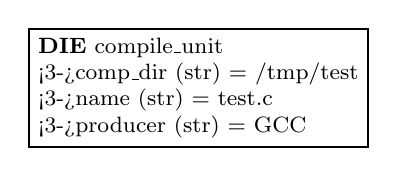
\begin{tikzpicture}
      \node [die] (CU) {
	\textbf{DIE} \tikz[remember picture,baseline=2pt,xshift=-1pt] \node [coordinate] (TYPE2) {};compile\_unit \\
      {\uncover<3->{\tikz[remember picture,baseline=1pt,xshift=0pt] \node [coordinate] (AT2) {};comp\_dir (str) = /tmp/test}} \\
      {\uncover<3->{name (str) = test.c}} \\
      {\uncover<3->{producer \tikz[remember picture,baseline=2pt] \node [coordinate,xshift=2mm] (FORM2) {};(str) = \tikz[remember picture,baseline=2pt] \node [coordinate] (HODN2) {};GCC}}
    };
    \end{tikzpicture}
  \end{textblock*}

  \onslide<1->

  \tikzstyle{mem} = [->,semithick,>=stealth']
  \begin{tikzpicture}[remember picture,overlay]
    \path[mem] (TYPE1) edge[out=0,in=190] (TYPE2);
    \path<3->[mem] (AT1) edge[out=5,in=230] (AT2);
    \path<4->[mem] (FORM1) edge[out=5,in=250] (FORM2);
    \path<5->[mem] (HODN1) edge[out=5,in=250] (HODN2);
  \end{tikzpicture}

\end{frame}

\begin{frame}[fragile]
  \frametitle{Hlavní DIE}

\begin{lstlisting}
DW_TAG_compile_unit
    DW_AT_producer              GNU C 4.7.2 20130108 [gcc-4_7-branch revision 195012]
    DW_AT_language              DW_LANG_C89
    DW_AT_name                  test.c
    DW_AT_comp_dir              /tmp/test
    DW_AT_low_pc                0x00000000
    DW_AT_entry_pc              0x00000000
    DW_AT_stmt_list             0x00000000
...
DW_TAG_subprogram
    DW_AT_external              yes(1)
    DW_AT_name                  main
    DW_AT_decl_file             0x00000001 /tmp/test/test.c
    DW_AT_decl_line             0x00000019
    DW_AT_prototyped            yes(1)
    DW_AT_type                  <0x0000005b>
    DW_AT_low_pc                0x00000000
    DW_AT_high_pc               0x0000011d
    DW_AT_frame_base            ...
    DW_AT_GNU_all_call_sites    yes(1)
    DW_AT_sibling               <0x00000770>
\end{lstlisting}

\end{frame}

\begin{frame}[fragile]
  \frametitle{Atributy DIE}

  \heading{Iterace přes všechny atributy v jednom DIE}\\
    \code{ptrdiff_t dwarf_getattrs(...)}
    \begin{itemize}
      \item \code{Dwarf_Die *die}: z \code{dwfl_nextcu}
      \item \code{int (*callback)(Dwarf_Attribute *, void *)}: vaše funkce,
        která se zavolá pro každý atribut v DIE
      \item \code{void *arg}: něco, co se předá do \code{callback} jako 2.\ 
        parametr
      \item \code{ptrdiff_t offset}: \code{0}
    \end{itemize}

  \pause
  \medskip

  \heading{Operace nad atributem}
  \begin{itemize}
    \item O co jde: \code{dwarf_whatattr(Dwarf_Attribute *attr)}
    \begin{itemize}
      \item Vrací \code{DW_AT_*} (\code{DW_AT_name} apod.)
    \end{itemize}

    \pause

    \item Typ obsahu: \code{dwarf_whatform(Dwarf_Attribute *attr)}
    \begin{itemize}
      \item Vrací \code{DW_FORM_*} (\code{DW_FORM_string} apod.)
    \end{itemize}

    \pause

    \item Obsah: \code{dwarf_form*(Dwarf_Attribute *attr)}
    \begin{itemize}
      \item Např.\ \code{dwarf_formstring}
    \end{itemize}
  \end{itemize}

\end{frame}

\begin{frame}[fragile]
  \frametitle{Atributy DIE -- příklad}

  \begin{lstlisting}[belowskip=0pt]
static int dump_die_attr(Dwarf_Attribute *attr, void *ptr)
{
  \end{lstlisting}
  \onslide<2->
  \begin{lstlisting}[aboveskip=0pt,belowskip=0pt]
  printf("AT=%x FORM=%x\n", dwarf_whatattr(attr), dwarf_whatform(attr));
  if (dwarf_whatform(attr) == DW_FORM_strp)
    printf("  name=%s\n", dwarf_formstring(attr));
  return DWARF_CB_OK;
  \end{lstlisting}
  \onslide<1->
  \begin{lstlisting}[aboveskip=0pt]
}

static void dump_dwfl(Dwfl *dwfl)
{
  Dwarf_Die *die = NULL;
  Dwarf_Addr bias;

  while ((die = dwfl_nextcu(dwfl, die, &bias))) {
    dwarf_getattrs(die, dump_die_attr, NULL, 0);
}
  \end{lstlisting}%stopzone

\end{frame}

\begin{frame}
  \frametitle{Úkol}

  \heading{Výpis atributů}
  \begin{enumerate}
    \item Definujte funkci (háček) pro \code{dwarf_getattrs}
    \item V ní vypište informace
    \begin{itemize}
      \item O jaký atribut jde (\code{dwarf_whatattr(attr)})
      \item Typ obsahu atributu (\code{dwarf_whatform(attr)})
      \item Adresu, pokud se jedná o typ \code{DW_AT_low_pc}
      \item Řetězec, pokud se jedná o typ obsahu \code{DW_FORM_string} nebo
	\code{DW_FORM_strp}
    \end{itemize}
    \item V těle cyklu \code{dwfl_nextcu} zavolejte \code{dwarf_getattrs}
    \item Přeložte a spusťte
  \end{enumerate}

\end{frame}

\begin{frame}
  \frametitle{Průchod skoro-stromem}

  \heading{Procházení okolních DIE}
  \begin{itemize}
    \item \code{int dwarf_child(Dwarf_Die *die, Dwarf_Die *result)}
    \begin{itemize}
      \item Do \code{result} vloží 1.\ potomka \code{die}
      \item Vrací 0 (OK), 1 (žádný potomek), -1 (chyba)
      \item \code{result} musí být ukazatel na lokální proměnnou
    \end{itemize}

    \pause

    \item \code{int dwarf_siblingof(Dwarf_Die *die, Dwarf_Die *result)}
    \begin{itemize}
      \item Do \code{result} vloží sourozence \code{die}
      \item Vrací 0 (OK), 1 (žádný sourozenec), -1 (chyba)
    \end{itemize}

  \end{itemize}

\end{frame}

\begin{frame}
  \frametitle{Úkol}

  \heading{Výpis potomků CU}
  \begin{enumerate}
    \item Vezměte 1.\ potomka od CU (\code{dwarf_child})
    \item Iterujte přes sourozence potomka (\code{dwarf_siblingof})
    \item Pro všechny potomky vypište typ DIE (\code{dwarf_tag})
    \begin{itemize}
      \item Nejprve zjistěte, které tam jsou
      \item Potom vypisujte v textové podobě
    \end{itemize}

    \iffimuni
    \item Rozšiřte na celý podstrom, nejen první úroveň
    \fi
    \item Přeložte a spusťte
  \end{enumerate}

\end{frame}
